\section{实现细节}
\label{appendix-imple}
\subsection{问题定义}
\label{appendix-imple-def}

\subsubsection{概述}
\label{appendix-imple-def-overview}

所提出的SparseAD兼容来自多模态传感器的输入，包括相机、毫米波雷达和激光雷达。本文将相机图像作为主要输入模态，同时可以进一步引入毫米波点云以获得额外性能提升。通常，将输入图像 $\textbf{I}_1,... ,\textbf{I}_{N_i}$ 联合表示为 $\textbf{I} \in \mathcal{R}^{N_i \times H \times W \times 3}$，其中 $N_i$ 表示输入图像数量；将输入点云表示为 $\mathbf{P} \in \mathcal{R}^{N_p \times {C_p}}$，其中 $N_p$ 表示输入点云中的点数，$C_p$ 是原始点云的维度，在nuScenes数据集中激光雷达为4，雷达为18。如 \cref{fig:arch} 所示，图像和点云通过不同编码器 $E_i$ 和 $E_p$ 编码到维度为 $C$ 的高维特征空间。将编码后的多模态传感器特征统一为传感器令牌 $\textbf{F}_t \in \mathcal{R}^{(N_i \times H \times W + N_p) \times C}$，表示如下：
\begin{equation}
{{\mathbf{F}}_t} = {\rm{Concat}}\left( {{\rm{Flatten(}}{{\mathbf{F}}_I}{\rm{),Flatten(}}{{\mathbf{F}}_P}{\rm{)}}} \right)
\end{equation}
其中
$$
\mathbf{F}_I = E_i(\mathbf{I}),\qquad\mathbf{F}_p = E_p(\mathbf{P})
$$

同样，传感器令牌的位置嵌入（PE）也通过拼接各模态令牌的PE获得。在SparseAD中，对图像特征和点云特征分别使用3D-PE和BEV-PE，其细节可参考PETR\cite{liu2022petr} 和CMT\cite{yan2023cross}。

在SparseAD中，使用多种查询（Query）实现对驾驶场景的稀疏表示并保持多任务能力。如 \cref{fig:arch} 所示，大多数查询可分为两类：一类是具有可学习权重的初始化查询，用于在训练中获取目标分布的先验特征；另一类是来自端到端多任务记忆库（EMMB）的记忆查询，用于传播各任务的时序信息以及将上游信息传递到下游任务。使用上标 $i$ 和 $m$ 分别表示可学习查询 $Q^i$ 和记忆查询 $Q^m$，将在后续部分介绍它们。注意，此处引入两层级记忆机制，其中场景级和实例级记忆的存储和更新策略不同，将在 \cref{appendix-imple-summary} 中详细描述。

\subsubsection{稀疏感知}
\label{appendix-imple-def-perception}

如 \cref{fig:dt-map-arch} 所示，在稀疏感知模块中，设置可学习的检测查询 $\mathbf{Q}^i_d\in \mathcal{R}^{N^i_d \times C}$ 和在线建图查询 $\mathbf{Q}^i_o\in \mathcal{R}^{N^i_o \times C}$，用于实现当前驾驶场景中障碍物和地图元素的基本感知，其中 $N^i_d$ 和 $N^i_o$ 分别为两种查询的数量。同时，来自EMMB的时序信息也被引入作为记忆查询，包括场景级记忆（检测记忆查询 $\mathbf{Q}^m_d\in \mathcal{R}^{N^m_d \times C}$ 和建图记忆查询 $\mathbf{Q}^m_o\in \mathcal{R}^{N^m_o \times C}$）以及作为实例级记忆的跟踪查询 $\mathbf{Q}^m_{t,T-1}\in \mathcal{R}^{N^m_i \times1\times C}$，其中 $N^m_d,N^m_o$ 分别为检测和在线建图记忆的长度，$N^m_i$ 为EMMB中的记忆实例数量，$T-1$ 表示上一帧。

最后，稀疏感知模块输出驾驶场景中障碍物（坐标、尺寸、ID、速度等）和地图元素（贝塞尔控制点、采样点等）的详细信息，以及对应的富含上下文的查询，这些信息被提供给下游的运动规划器并更新到EMMB中供未来帧的感知使用。稀疏感知模块的实现细节将在 \cref{appendix-imple-perception} 中详细描述。

\subsubsection{运动规划器}
\label{appendix-imple-def-motionplanner}

如 \cref{fig:fore-arch} 所示，在运动规划器中统一了对周围智能体和自车的多模态运动预测。由于运动查询的数量随实例数量变化，为所有运动查询设置了一个共享的可学习嵌入 $\mathbf{E}_n \in \mathcal{R}^{1\times C}$。通过MLP对每个实例的历史轨迹 $\tau_h$ 进行编码，随后经过交叉注意力层聚合该实例的历史感知信息（如跟踪查询 $\mathbf{Q}^m_{t}\in \mathcal{R}^{N^m_i \times M\times C}$，其中 $M$ 是实例的最大历史长度），并与可学习嵌入 $\mathbf{E}_n$ 结合作为运动查询 $\mathbf{Q}^i_n \in \mathcal{R}^{N^m_i \times C}$ 的初始化。特别地，仅对自车历史轨迹 $\tau_{eh}$ 进行编码，并与特殊的自车嵌入 $\mathbf{E}_e \in \mathcal{R}^{1\times C}$ 结合作为自车查询 $\mathbf{Q}^i_e \in \mathcal{R}^{1 \times C}$ 的初始化。类似地，引入实例的记忆运动查询 $\mathbf{Q}^m_n \in \mathcal{R}^{N^m_i \times M\times C}$、自车记忆运动查询 $\mathbf{Q}^m_e \in \mathcal{R}^{1 \times M\times C}$，以及来自稀疏感知的当前帧智能体稀疏表示 $\mathbf{Q}^m_{t,T}\in \mathcal{R}^{N^m_i \times1\times C}$ 和地图元素 $\mathbf{Q}_{o}\in \mathcal{R}^{N^i_o \times C}$ 作为令牌，与运动查询和自车查询充分交互，生成高质量的多模态运动预测轨迹 $\hat{\tau}$。随后，自车查询进一步输入到规划优化器中，充分考虑安全和运动学约束，最终生成安全可靠的自车轨迹规划 $\hat{\tau_e}$。运动规划器的实现细节将在 \cref{appendix-imple-motionplanner} 中详细描述。

\subsection{稀疏感知}
\label{appendix-imple-perception}

如 \cref{fig:dt-map-arch} 所示，稀疏感知模块将传感器令牌 $\textbf{F}_t$ 作为输入，查询通过两个结构相同的时序解码器\cite{wang2023exploring} 以及对应的检测\&跟踪头和贝塞尔地图头解码相应的感知结果。参照StreamPETR\cite{wang2023exploring}，时序解码器的输入和输出可表示如下：
\begin{equation}
Q^c = {\rm{Temporal}}\_{\rm{Decoder}}({\textit{Query}},{\textit{Tokens}},{\textit{Memory}})
\label{eq:temporal-decoder}
\end{equation}

在SparseAD中，通过利用不同的输入，\cref{eq:temporal-decoder} 可同时应用于检测\&跟踪和在线建图任务。对于检测\&跟踪，从场景级的检测记忆查询 $\mathbf{Q}^m_{d}$ 中选择最新更新的Top $K_d$ 个查询 $\mathbf{Q}^m_{dk} \in \mathcal{R}^{K_d \times C}$，连同可学习检测查询 $\mathbf{Q}^i_{d}$ 和实例级的跟踪查询 $\mathbf{Q}^m_{t,T-1}$，作为时序解码器的\textit{Query}输入。所有检测记忆查询 $\mathbf{Q}^m_{d}$ 和传感器令牌 $\textbf{F}_t$ 分别作为\textit{Memory}和\textit{Tokens}输入。综上，检测\&跟踪任务的解码器可表示如下：
\begin{equation}
\mathbf{Q}^c_d = {\rm{Temporal}}\_{\rm{Decoder}}(\text{Concat}(\mathbf{Q}^m_{dk},\mathbf{Q}^i_{d},\mathbf{Q}^m_{t,T-1}),\textbf{F}_t,\mathbf{Q}^m_{d})
\label{eq:det-decoder}
\end{equation}
其中 $\mathbf{Q}^c_d \in \mathcal{R}^{(K_d+N^i_d+N^m_i)\times C}$ 是当前帧时序解码器输出的检测\&跟踪查询。这里省略了 $\mathbf{Q}^m_{t,T-1}$ 的第二维（为1）以简化描述。

在线建图任务的解码器输入与 \cref{eq:det-decoder} 类似但更简单，因为地图元素不需要在帧间关联和分配唯一ID。这里从场景级的建图记忆查询 $\mathbf{Q}^m_{o}$ 中选择最新更新的Top $K_o$ 个查询 $\mathbf{Q}^m_{ok} \in \mathcal{R}^{K_o \times C}$，连同可学习在线建图查询 $\mathbf{Q}^i_{o}$ 作为时序解码器的\textit{Query}输入。所有建图记忆查询 $\mathbf{Q}^m_{o}$ 和传感器令牌 $\textbf{F}_t$ 分别作为\textit{Memory}和\textit{Tokens}输入。综上，在线建图任务的解码器可表示如下：
\begin{equation}
\mathbf{Q}^c_o = {\rm{Temporal}}\_{\rm{Decoder}}(\text{Concat}(\mathbf{Q}^m_{ok},\mathbf{Q}^i_{o}),\textbf{F}_t,\mathbf{Q}^m_{o})
\end{equation}
其中 $\mathbf{Q}^c_o \in \mathcal{R}^{(K_o+N^i_o)\times C}$ 是当前帧时序解码器输出的在线建图查询。

对于 $\mathbf{Q}^c_d$，SparseAD使用与其他DETR类检测器\cite{liu2022petr,yan2023cross,jiang2023far3d,zhang2023fully} 类似的流行检测\&跟踪头，将其解码为由位置、尺寸、偏航角和速度组成的3D边界框。对于 $\mathbf{Q}^c_o$，参照BeMapNet\cite{qiao2023end}，SparseAD将稀疏地图元素视为分段贝塞尔曲线，并利用贝塞尔地图头为每个查询回归贝塞尔曲线参数，如显式控制点、隐式控制点、分段数和置信度等。特别地，为方便下游任务直观获取地图元素的准确位置，基于解码的贝塞尔曲线参数在每个地图元素的曲线上均匀采样 $S$ 个点。具体而言，给定系数为 $c$ 的一段贝塞尔曲线，可按下式在任何位置进行采样：

\begin{equation}
p(t)=\sum_{i=0}^n b_{i, n}(t) c_i, t \in[0,1]
\label{eq:bezier_eq_1}
\end{equation}
其中
\begin{equation}
b_{i, n}(t)=\left(\begin{array}{c}
n \\
i
\end{array}\right) t^i(1-t)^{n-i}, i=0, \ldots, n
\label{eq:bezier_eq_2}
\end{equation}
其中 $n$ 是贝塞尔曲线的阶数。通过采样，可以得到地图曲线点 $\mathbf{P}^c_o\in\mathcal{R}^{(K_o+N^i_o)\times S \times 2}$，将在下游任务中使用。

\subsection{运动规划器}
\label{appendix-imple-motionplanner}

如 \cref{fig:fore-arch} 所示，在运动规划器中，初始化运动查询 $\mathbf{Q}^i_n$ 和自车查询 $\mathbf{Q}^i_e$，以充分利用稀疏感知提供的先验信息和EMMB中的时序信息。

在运动规划器中，将 $\mathbf{Q}^c_d \in \mathcal{R}^{(K_d+N^i_d+N^m_i)\times C}$ 对应的所有 $K_d+N^i_d+N^m_i$ 个障碍物视为实例并参与推理。因此，运动规划器中的实例数量为 $N^c_i = K_d+N^i_d+N^m_i$。与记忆实例数量 $N^m_i$ 相比，为来自稀疏感知的新生 $K_d+N^i_d$ 个实例设置虚拟历史信息。为便于描述，下文不再区分新生实例和记忆实例，仅将记忆实例数 $N^m_i$ 替换为当前实例数 $N^c_i$。

从EMMB中，可以获取所有智能体和自车的历史位置信息 $\mathbf{P}^m_i\in\mathcal{R}^{N^c_i \times M \times 3}$ 和 $\mathbf{P}^m_e\in\mathcal{R}^{1 \times M \times 3}$。设置一个共享MLP对智能体和自车的历史轨迹进行编码，获得历史轨迹嵌入 $\textbf{H}_i\in\mathcal{R}^{N^c_i \times C}$ 和 $\textbf{H}_e\in\mathcal{R}^{1 \times C}$：
\begin{equation}
{{\mathbf{H}}_i} = {\rm{MLP}}({\mathbf{P}}_i^m), {{\mathbf{H}}_e} = {\rm{MLP}}({\mathbf{P}}_e^m)
\end{equation}

对于每个实例，进一步利用交叉注意力聚合历史感知信息：
\begin{equation}
{{\mathbf{H}}_{pi}} = {\rm{MHCA}}({{\mathbf{H}}_i},{\mathbf{Q}}_t^m)
\end{equation}
其中MHCA表示多头交叉注意力\cite{vaswani2017attention}，$\textbf{H}_{pi}\in\mathcal{R}^{N^c_i \times C}$ 是实例的历史嵌入。同时为运动查询初始化设置一个共享的可学习嵌入，为自车查询单独设置一个可学习嵌入。综上，运动规划器中的运动查询和自车查询可通过以下方式获得：
\begin{equation}
{\mathbf{Q}}_n^i = {{\mathbf{H}}_{pi}} + {{\mathbf{E}}_n},{\mathbf{Q}}_e^i = {{\mathbf{H}}_e} + {{\mathbf{E}}_e}
\end{equation}

在运动规划器的运动预测部分，自车查询被视为与运动查询等同，如 \cref{fig:fore-arch} 所示。为便于描述，在运动预测器的交互中使用运动查询 $\mathbf{Q}_n^i$ 指代运动查询 $\mathbf{Q}_n^i$ 和自车查询 $\mathbf{Q}_e^i$，使用记忆运动查询 $\mathbf{Q}_n^m$ 指代记忆运动查询 $\mathbf{Q}_n^m$ 和记忆自车查询 $\mathbf{Q}_e^m$。

使用K-Means方法在nuScenes \textit{train} 集中对智能体未来轨迹进行聚类，生成 $\mathcal{K}$ 个共享轨迹锚点。将它们映射到高维特征嵌入，并与运动查询结合形成多模态运动查询 $\mathbf{Q}_{mn}^i \in \mathcal{R}^{N^c_i\times \mathcal{K} \times C}$。然而，为简化描述，此处忽略运动查询的模态，仍使用 $\mathbf{Q}_{n}^i$ 作为运动查询的表示。

运动预测器由N个Transformer层组成，每层包括三种智能体与驾驶场景之间的交互：智能体-记忆、智能体-地图和智能体-社交。对于运动查询 $\mathbf{Q}_{n}^i$，其与记忆运动查询 $\mathbf{Q}_{n}^m$ 以及当前帧的检测跟踪查询 $\mathbf{Q}_{d}^c$ 和在线建图查询 $\mathbf{Q}_{o}^c$ 的交互可表示如下：
\begin{equation}
\mathbf{Q}_{n}^c = \text{MHCA}(\text{MHSA}(\mathbf{Q}_{n}^i),\mathbf{Q}_{n}^m / \mathbf{Q}_{d}^c/ \mathbf{Q}_{o}^c)
\end{equation}
其中 $\mathbf{Q}_{n}^c \in \mathcal{R}^{N^c_i \times C}$ 是当前帧更新后的运动查询，MHSA表示多头自注意力\cite{vaswani2017attention}。类似地，$\mathbf{Q}_{e}^c \in \mathcal{R}^{1 \times C}$ 表示当前帧更新后的自车查询。

针对上述智能体与记忆运动查询之间的交互，设计了时间位置编码（Temporal PE）来对齐同一智能体在不同时间步上的预测轨迹。智能体 $i$ 在时间T对未来 $L$ 步的运动预测轨迹可表示为 ${\cal F}_T^i = \{ {{\mathbf{v}}_{\mathbf{1}}},...,{{\mathbf{v}}_L}\}$，其中 $\mathbf{v}\in \mathcal{R}^3$ 是3D空间中的位置。记忆中的历史预测轨迹可表示为 $\left\{ {{\cal F}_{T - 1}^i,...,{\cal F}_{T - M}^i} \right\}$，其中 $M$ 是记忆最大长度。为简化问题，假设历史预测轨迹已转换到当前自车坐标系。对于智能体 $i$，记忆运动查询的时间位置编码 $\mathbf{E}_{n}^m$ 和当前运动查询的时间位置编码 $\mathbf{E}_{n}^c$ 可表示为：
\begin{equation}
\mathbf{E}_{n}^m = \sum\limits_{k = 1}^N {{\rm{ML}}{{\rm{P}}_k}({\rm{Cat}}(\{ {{\mathbf{v}}_j} - {{\mathbf{v}}_k}|j \ge k,{\mathbf{v}} \in {\cal F}_{T - k}^i\} ))}
\label{eq:ts_align_pe_memory}
\end{equation}

\begin{equation}
\mathbf{E}_{n}^c = \sum\limits_{k = 1}^N {{\rm{ML}}{{\rm{P}}_k}({\rm{Cat}}(\{ {{\mathbf{v}}_j} - {{\mathbf{v}}_0}|j \le M - k,{\mathbf{v}} \in {\cal F}_T^i\} ))}
\label{eq:ts_align_pe_agent}
\end{equation}

针对上述智能体与在线建图查询之间的交互，设计了曲线位置编码（Curve PE）来精确描述稀疏地图元素的位置信息。对于在线建图查询 $\mathbf{Q}_{o}^c$，曲线位置编码 $\mathbf{E}^c_o$ 可表示为：
\begin{equation}
\mathbf{E}^c_o = \sum\limits_{k = 1}^J {{\rm{ML}}{{\rm{P}}}(\text{Flatten}(\mathbf{P}^c_o) )}
\end{equation}
其中 $\mathbf{P}^c_o$ 是通过 \cref{eq:bezier_eq_1} 和 \cref{eq:bezier_eq_2} 获得的采样点。

针对上述智能体与社交（即跟踪查询）之间的交互，使用BEV位置编码（BEV PE）来描述场景中其他智能体的位置信息，该方法由CMT\cite{yan2023cross} 提出。

更新后的运动查询 $\mathbf{Q}_{n}^c$ 将用于解码每个智能体的多模态轨迹。参照流行方法\cite{shi2022motion,shi2024mtr++,zhou2022hivt}，SparseAD在训练过程中仅监督多模态结果中与真实轨迹最接近的轨迹。

{\small
\begin{algorithm}[H]
\captionsetup{font=tiny}
  \KwResult{智能体与自车的纵向和横向关系}
  $A$ \tcp*[h]{智能体真实未来轨迹，形状为 (F, T, N, 3)}\\
  $E$ \tcp*[h]{自车真实未来轨迹，形状为 (T, N, 3)}\\
  $LoC\leftarrow None$ \tcp*[h]{初始化智能体纵向关系}\\
  $LaC\leftarrow None$ \tcp*[h]{初始化智能体横向关系}\\
  $E_{speedup}$ \tcp*[h]{基于自车真实未来轨迹生成加速轨迹}\\
  $E_{speeddown}$ \tcp*[h]{基于自车真实未来轨迹生成减速轨迹}\\

  \For{$i\leftarrow 0$ \KwTo \texttt{F}}{
    \For{$t\leftarrow 0$ \KwTo T\texttt{F}}{
        \tcp{检查与自车轨迹的横向关系}
        \If{$(A[i,t],E[t])$ 的横向距离 $< thresh$}{
            $LaC[i] = Left$ 若 $A[i,t]$ 在 $E[t]$ 左侧，否则 $Right$
        }
        \tcp{检查与加速轨迹的纵向关系}
        \If{$(A[i,t],E_{speedup}[t])$ 的纵向距离 $< thresh$}{
            $LoC[i] = Front$
        }
        \tcp{检查与减速轨迹的纵向关系}
        \If{$(A[i,t],E_{speeddown}[t])$ 的纵向距离 $< thresh$}{
            $LoC[i] = Back$
        }
    }
  }
  \caption{纵向和横向关系生成}
\label{alg:relationship}
\end{algorithm}}

遵循自车查询与驾驶指令之间的交互，本文认为规划轨迹在规划优化器中应遵循一定的场景约束。与先前工作\cite{jiang2023vad} 一致，引入了自车-地图、自车-智能体和自车-运动学约束。利用其他智能体和自车的未来轨迹来描述它们在纵向和横向方向上的相互约束。关于自车-智能体关系约束的更多细节，请参阅 \cref{alg:relationship}。

在生成这些标签后，在规划优化器中进行一系列监督，如 \cref{sec:motion_planner} 所述，最终输出规划结果。

\subsection{帧总结}
\label{appendix-imple-summary}

在稀疏感知和运动规划器推理之后，所提出的SparseAD将来自多任务的信息总结并更新到EMMB中，为未来帧提供高质量的先验信息。存储每个任务的更新后查询（如检测\&跟踪 $\mathbf{Q}^c_d$、在线建图 $\mathbf{Q}^c_o$、运动 $\mathbf{Q}^c_n$ 和规划 $\mathbf{Q}^c_e$）以及对应的解码信息（如3D边界框、贝塞尔曲线控制点、采样点、多模态预测轨迹和自车规划轨迹等）到EMMB中。与常见流程一致，当EMMB中的记忆查询传播到下一帧时，对EMMB中的所有位置信息进行必要的自车变换，以消除自车运动的影响。

具体而言，将 $\mathbf{Q}^c_d$ 中置信度Top $K_d$ 的查询 $\mathbf{Q}^c_{dk} \in \mathcal{R}^{K_d\times C}$ 作为场景级检测查询存储到EMMB中。同时，根据阈值 $\mathcal{T}$ 选择 $\mathbf{Q}^c_d$ 中的高置信度查询作为实例级跟踪查询 $\mathbf{Q}^c_t$，相应的实例将被分配唯一ID。与此同时，与跟踪查询对应的下游查询（即运动查询）将作为实例级记忆存储，而未分配ID的检测查询对应的下游查询将被丢弃。

\begin{figure}[tb]
  \centering
  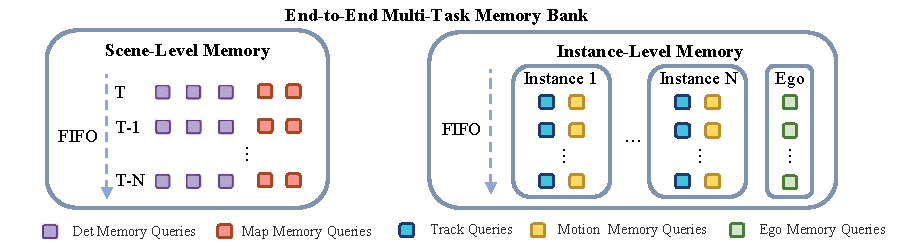
\includegraphics[width=0.7\linewidth]{Figures/EMMB-Figure}
  \caption{端到端多任务记忆库（EMMB）示意图。}
  \label{fig:emmb}
\end{figure}

SparseAD提出的端到端多任务记忆库（EMMB）如 \cref{fig:emmb} 所示。SparseAD利用两种不同的策略维护EMMB中的场景级和实例级记忆。对于场景级记忆，以帧为单位存储并遵循先进先出（FIFO）原则。对于实际流数据，可以假设场景级记忆始终存储前 $M$ 帧的感知信息。相比之下，实例级记忆以实例为单位存储，对同一实例的记忆遵循FIFO原则，而实例本身没有生命周期限制。当稀疏感知模块检测到新的障碍物时，将新实例添加到实例级记忆中存储其对应信息。当实例连续多帧未被检测到时（例如消失、漏检或ID切换），该实例及其所有对应的历史信息将被移除。两层级记忆设计使SparseAD能够充分利用全局（场景）和局部（实例）时序信息，实现强大的端到端自动驾驶性能。
